\section{Results}

\begin{figure*}[!t]
  \centering
  % Replace with the final bar chart (native aspect ratio approx 2.8:1):
  % 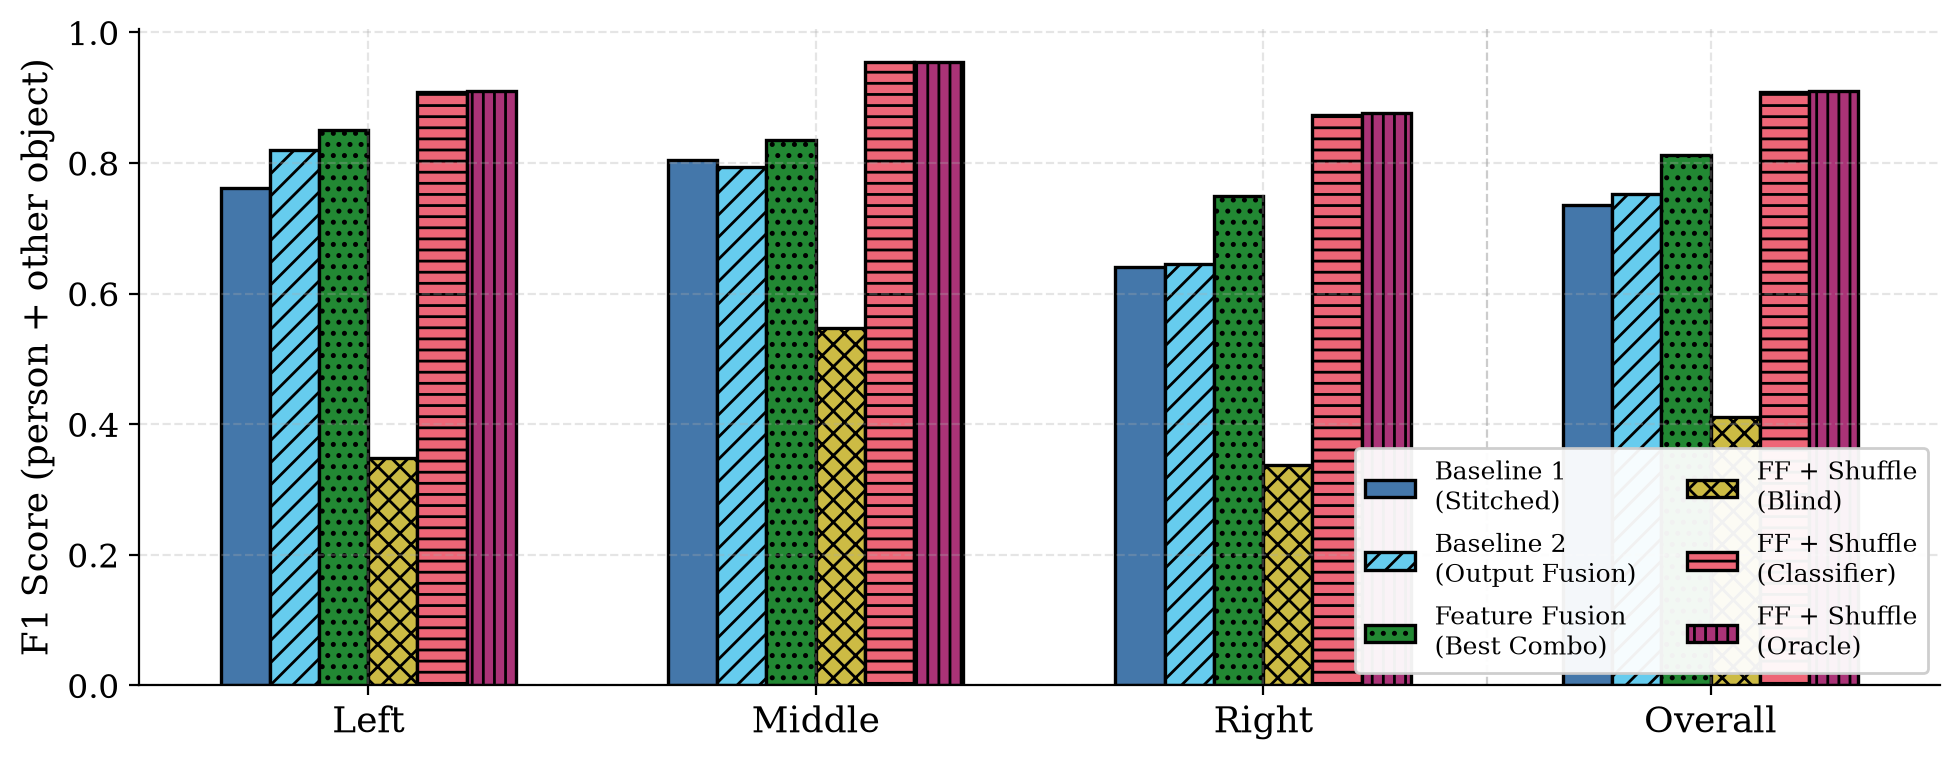
\includegraphics[width=\textwidth]{fig1_macro_f1_color.png}
  \figplaceholder[\textwidth]{0.13\textheight}{%
    \textbf{Bar chart 1: architecture comparison.}\\[0.3em]
    Per-class $F_1$ by camera direction for the four architectures
    (\texttt{fig1\_macro\_f1\_color.png}).}
  \caption{Per-class $F_1$ by camera direction for the obstruction-detection
  architectures. Baselines and Feature Fusion are evaluated on the validation
  set; Feature Fusion with shuffle correction (blind, classifier, oracle) is
  evaluated on the held-out test set.}
  \label{fig:arch_f1}
\end{figure*}

\subsection{Navigability Estimation Performance}

Figure~\ref{fig:arch_f1} compares the four architectures using per-class $F_1$
broken down by camera direction. All models estimate the three navigability
states well above chance from the raw $32\times24$ thermal tiles, confirming that
directional navigability is recoverable from ultra-low-resolution thermal sensing
alone. On the validation set, Feature Fusion is the strongest of the calibrated
(non-shuffled) models, reaching overall per-class $F_1$ of roughly $0.81$
(clear), $0.83$ (person), and $0.80$ (other object). The stitched-panorama and
output-fusion baselines trail it, with overall $F_1$ near $0.73$--$0.78$, and
both show markedly weaker person detection on the right camera, where the useful
thermal signal is sparsest.

\subsection{Fusion Strategy Analysis}

Feature-level fusion consistently outperforms both pixel-level stitching and
decision-level output fusion. Mixing intermediate feature maps across cameras at
every backbone depth preserves cross-camera spatial detail that the alternatives
discard: the stitched panorama warps and blurs the already-coarse thermal signal
before the model sees it, while output fusion only combines low-dimensional,
already-classified logits. Feature fusion costs extra backbone passes, but on
these ultra-low-resolution tiles the accuracy gain justifies the compute, so we
adopt it as the reference architecture for the robustness study.

\begin{figure}[!b]
  \centering
  % Replace with the final bar chart (native aspect ratio approx 1.75:1):
  % 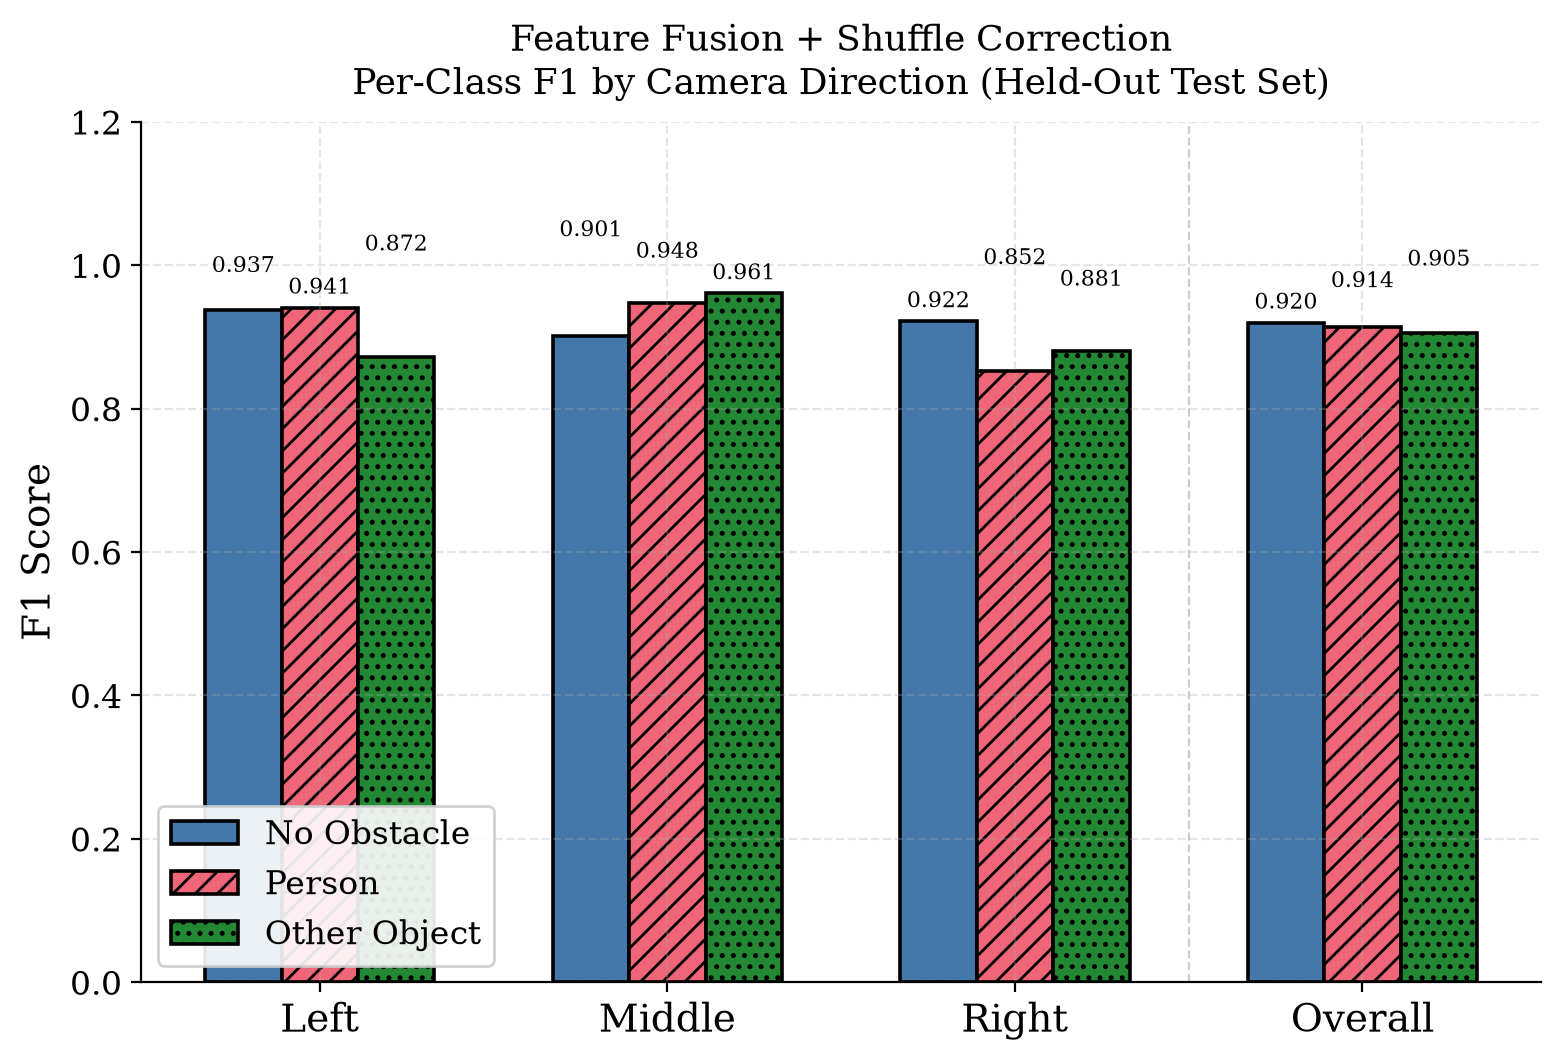
\includegraphics[width=\linewidth]{fig2_ff_per_class_color.png}
  \figplaceholder[\linewidth]{0.11\textheight}{%
    \textbf{Bar chart 2: shuffle-corrected Feature Fusion.}\\[0.3em]
    Per-class $F_1$ by direction and overall
    (\texttt{fig2\_ff\_per\_class\_color.png}).}
  \caption{Per-class $F_1$ of Feature Fusion with classifier-based shuffle
  correction on the held-out test set, broken down by camera direction (left,
  middle, right) and overall.}
  \label{fig:ff_shuffle}
\end{figure}

\subsection{Camera Arrangement Robustness}

Figure~\ref{fig:ff_shuffle} reports Feature Fusion under permuted camera slots on
the held-out test set. Without correction (blind), shuffling the physical
camera-to-slot assignment collapses performance to overall per-class $F_1$ near
$0.40$--$0.42$, confirming that the fixed-slot projection layers learn a
positional dependence that does not survive re-arrangement. The lightweight
camera-identity classifier, which re-sorts tiles to their most likely directions
before the unmodified model, restores overall $F_1$ to roughly $0.90$--$0.92$
across all three classes---matching the ground-truth oracle re-sort to within
rounding. Once tiles are routed to the correct directions the underlying features
are themselves directionally meaningful, so the system is robust to camera
placement rather than overfit to which camera feeds which input channel.
